% https://tex.stackexchange.com/a/353676
\documentclass{beamer}
\usepackage{tikz}

\begin{document}
    \begin{frame}<1-3>[label=foo]{Contents}
        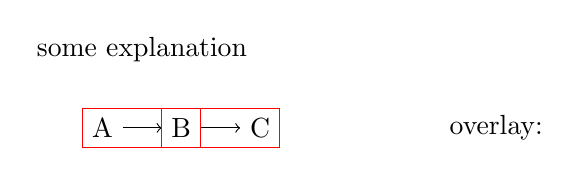
\begin{tikzpicture}
            \node at (5,0) {overlay: \insertoverlaynumber};
            \node (a) at (0,0) {A};
            \node (b) at (1,0) {B};
            \node (c) at (2,0) {C};
            \pause % -------------------------------------
            \draw [->] (a) -- (b);
            \draw [->] (b) -- (c);
            \pause %--------------------------------------
            \visible<+>{
                \node at (0.5,1) {some explanation};
            }
            % --------------------------------------------
            \visible<+>{
                \draw [red] 
                    (a.south west) rectangle (b.north east);
            }
            % --------------------------------------------
            \visible<+>{
                \draw [red] 
                    (a.south west) rectangle (b.north east);
            }
            % --------------------------------------------
            \visible<+>{
                \draw [red] 
                    (b.south west) rectangle (c.north east);
            }
        \end{tikzpicture}
    \end{frame}

    \begin{frame}
        other frame
    \end{frame}

    \againframe<4>{foo}

    \begin{frame}
        yet other frame
    \end{frame}


\end{document}
